\documentclass[11pt,a4paper]{article}
\usepackage[utf8]{inputenc}
\usepackage[T1]{fontenc}
\usepackage{lmodern}
\usepackage[top=1.8cm,bottom=1.8cm,left=1.9cm,right=1.9cm]{geometry}
\usepackage{amsmath,amssymb}
\usepackage{booktabs}
\usepackage{graphicx}
\usepackage{subcaption}
\usepackage{hyperref}
\usepackage{xcolor}
\usepackage{titlesec}
\usepackage{tabularx}
\usepackage{float}

% Ajuste de tolerâncias de floats para distribuição coesa de figuras e tabelas
\renewcommand{\topfraction}{0.88}
\renewcommand{\bottomfraction}{0.85}
\renewcommand{\textfraction}{0.12}
\renewcommand{\floatpagefraction}{0.75}

\hypersetup{
    colorlinks=true,
    linkcolor=blue!70!black,
    citecolor=blue!70!black,
    urlcolor=blue!70!black
}

\titleformat{\section}{\large\bfseries}{\thesection.}{0.5em}{}
\titleformat{\subsection}{\normalsize\bfseries}{\thesubsection.}{0.5em}{}
\titlespacing*{\section}{0pt}{1.0ex plus 0.4ex minus .2ex}{0.4ex}
\titlespacing*{\subsection}{0pt}{0.8ex plus 0.3ex minus .2ex}{0.3ex}

\setlength{\parskip}{0.33em}
\setlength{\parindent}{0pt}

\begin{document}

\begin{center}
    {\LARGE \textbf{Projeto 1: Regressão Não Linear com Perceptron Multicamadas e Estudo de Ablação de Regularizadores}} \\[0.4em]
    {\large Disciplina: Introdução às Redes Neurais Artificiais} \\[0.3em]
    \textbf{Autor(es):} Gabriel Leal Bonavina (RA: 168.858) \\[0.2em]
    \textbf{Repositório / Código Reprodutível:} \url{https://github.com/gbonavina/projeto-1-rna} 
\end{center}
\vspace{-0.4em}
\hrule
\vspace{0.8em}

\section{Configuração Experimental e Reprodutibilidade Metodológica}

\subsection{Caracterização dos Dados, Particionamento e Pré-processamento}
O problema sob investigação consiste no mapeamento funcional não linear univariado a partir de um conjunto sintético contendo $N = 300$ pares ordenados $(x, y)$. A variável independente distribui-se no intervalo contínuo $x \in [0, 10]$, enquanto a variável dependente assume valores no domínio $y \in [-1{,}49,\, 2{,}66]$, apresentando média amostral $\mu_y \approx 0{,}47$ e desvio-padrão $\sigma_y \approx 0{,}73$. O coeficiente de correlação linear de Pearson calculado sobre a totalidade das amostras é praticamente nulo ($\mathrm{corr}(x,y) \approx -0{,}007$), atestando a completa ineficácia de regressores lineares para a predição da variável resposta. Não obstante a ausência de correlação linear, os dados contêm expressiva dependência funcional determinística sobreposta por ruído, como evidencia o ajuste de um polinômio global de quarto grau, capaz de explicar aproximadamente 17\% da variância total ($R^2 \approx 0{,}17$).

Com o intuito deliberado de induzir sobreajuste (\textit{overfitting}) e estabelecer um ambiente propício para a avaliação comparativa de mecanismos de regularização, adotou-se um protocolo de particionamento assimétrico estrito na proporção de 10\% para treinamento, 10\% para validação e 80\% para teste independente (\texttt{random\_state=123}). Tal procedimento resultou em partições com 30 amostras de treino, 30 de validação e 240 de teste. A restrição drástica do subconjunto de ajuste a meras 30 observações impõe um regime severo de escassez amostral frente à capacidade representacional da rede neural, garantindo que o modelo memorize as oscilações estocásticas do treino caso não seja devidamente restringido.

Para resguardar a integridade metodológica e evitar o vazamento espúrio de informação entre partições (\textit{data leakage}), a padronização das variáveis foi conduzida por meio do operador \textit{StandardScaler}, estimando-se os parâmetros de centralidade e escala ($\mu$ e $\sigma$) com base unicamente nas 30 amostras da partição de treino. As transformações afins correspondentes foram aplicadas estaticamente aos conjuntos de validação e teste. O treinamento do modelo foi executado com o alvo $y$ padronizado, regime no qual uma perda de Erro Quadrático Médio unitária ($\mathrm{MSE} \approx 1{,}0$) corresponde à predição trivial da média amostral. As avaliações de generalização e as métricas residuais finais foram convertidas de volta à escala dimensional original de $y$ via transformação inversa (\textit{inverse\_transform}), preservando o significado físico das grandezas mensuradas.

\subsection{Arquitetura da MLP Baseline e Otimização Numérica}
A rede neural padrão (\textit{Baseline Vanilla}) foi configurada como um Perceptron Multicamadas (\textit{Multi-Layer Perceptron} -- MLP) com três camadas ocultas densas de 100 neurônios cada, resultando na topologia sequencial $1 \to 100 \to 100 \to 100 \to 1$. Essa formulação soma 20.501 parâmetros livres ajustáveis entre pesos sinápticos e termos de polarização (\textit{biases}), constituindo um sistema altamente superparametrizado em relação às 30 restrições do conjunto de treino ($p \gg N$). As camadas intermediárias utilizam a função de ativação linear retificada (\textit{Rectified Linear Unit} -- ReLU), proporcionando capacidade de aproximação não linear contínua por partes, ao passo que a camada de saída emprega ativação linear, apropriada para regressão contínua irrestrita.

A otimização dos parâmetros foi realizada mediante o algoritmo de Gradiente Descendente Estocástico (SGD puro), sem termo de momento ($\beta = 0$), sem decaimento de pesos ($\lambda = 0$) e sem regularização estocástica por descarte de ativações ($p = 0$). Definiu-se uma taxa de aprendizado constante $\eta = 0{,}01$, tamanho de minilote de 8 amostras (\textit{batch size}) e função de custo do Erro Quadrático Médio ($\mathrm{MSELoss}$). O treinamento estendeu-se por um orçamento exaustivo de 10.000 épocas. A especificação detalhada da parametrização baseline encontra-se sintetizada na Tabela~\ref{tab:baseline_hiper}.

\begin{table}[htbp]
\centering
\small
\renewcommand{\arraystretch}{1.15}
\caption{Especificação hiperparamétrica da arquitetura MLP de referência (\textit{Baseline Vanilla}).}
\label{tab:baseline_hiper}
\begin{tabularx}{\textwidth}{>{\bfseries\raggedright\arraybackslash}p{4.8cm} X}
\toprule
Hiperparâmetro / Componente & Configuração Experimental Adotada \\
\midrule
Topologia Estrutural & Entrada (1) $\to$ Densa (100) $\to$ Densa (100) $\to$ Densa (100) $\to$ Saída (1) \\
Funções de Ativação & ReLU nas camadas intermediárias / Linear na camada de saída \\
Volume de Parâmetros & 20.501 coeficientes ajustáveis (pesos sinápticos e polarizações) \\
Algoritmo Otimizador & Gradiente Descendente Estocástico (SGD padrão, $\eta = 0{,}01$, $\beta = 0$) \\
Tamanho do Minilote & 8 amostras por iteração estocástica \\
Critério de Perda & Erro Quadrático Médio (\textit{Mean Squared Error} -- MSE) \\
Orçamento de Treinamento & 10.000 épocas completas \\
Particionamento dos Dados & 10\% Treino (30) / 10\% Validação (30) / 80\% Teste (240) \\
Semente Aleatória (\textit{Seed}) & 123 (\texttt{random\_state}) \\
\bottomrule
\end{tabularx}
\end{table}

A convergência empírica consolida o diagnóstico de superajuste planejado: ao final das 10.000 épocas, o \textit{baseline} atinge um $\mathrm{MSE}$ de treino padronizado de $0{,}032$, ao passo que a perda sobre as 30 amostras de validação atinge $0{,}641$, culminando em um expressivo hiato de generalização de $0{,}609$. A Tabela~\ref{tab:train_val} detalha o comportamento comparativo de treino, validação e hiato entre o modelo base e as variações submetidas à ablação.

\begin{table}[htbp]
\centering
\small
\renewcommand{\arraystretch}{1.2}
\caption{Valores finais de MSE no treino e na validação após 10.000 épocas (alvo $y$ padronizado). O hiato (\textit{gap}) corresponde à diferença $\mathrm{MSE}_{\mathrm{val}} - \mathrm{MSE}_{\mathrm{treino}}$.}
\label{tab:train_val}
\begin{tabular}{l c c c}
\toprule
\textbf{Modelo / Variação} & \textbf{MSE Treino} & \textbf{MSE Validação} & \textbf{Hiato de Generalização} \\
\midrule
Baseline Vanilla (SGD puro) & 0{,}032 & 0{,}641 & 0{,}609 \\
Dropout ($p=0{,}05$) & 0{,}222 & 0{,}670 & 0{,}448 \\
Regularização L2 ($\lambda=10^{-3}$) & 0{,}053 & 0{,}601 & 0{,}548 \\
Regularização L1 ($\lambda=10^{-3}$) & 0{,}254 & 0{,}791 & 0{,}537 \\
Otimizador com Momentum ($\beta=0{,}9$) & 0{,}039 & 0{,}636 & 0{,}596 \\
\bottomrule
\end{tabular}
\end{table}

\section{Dinâmica de Treinamento, Otimização e Convergência Empírica}

A evolução temporal das curvas de perda reflete diretamente a interação entre a geometria da superfície de custo, a estocasticidade do algoritmo de otimização e as penalidades impostas à capacidade da rede. Na Figura~\ref{fig:loss_baseline}, observa-se a trajetória completa de aprendizado do modelo baseline. Enquanto a perda de treino decai de forma suave e monotônica, reduzindo-se de aproximadamente $1{,}0$ no início até o piso assintótico de $0{,}032$ próximo à época 4.000, a curva de validação exibe extrema turbulência estocástica entre as épocas 500 e 4.000. Essa instabilidade traduz-se em oscilações contínuas de alta frequência e picos abruptos que ultrapassam a marca de $2{,}0$ (notadamente ao redor da época 3.800). Essa volatilidade decorre da conjunção entre minilotes diminutos de 8 amostras sobre uma partição restrita a 30 elementos, gerando gradientes de alta variância que provocam perturbações nas predições de pontos ainda não vistos. A bifurcação definitiva entre as curvas consolida-se em torno da época 1.500: a partir desse limiar, a validação estagna permanentemente na faixa de $0{,}60$ a $0{,}70$, evidenciando a memorização dos dados de treino em detrimento da capacidade de extrapolação.

\begin{figure}[htbp]
\centering
\begin{subfigure}[t]{0.48\textwidth}
    \centering
    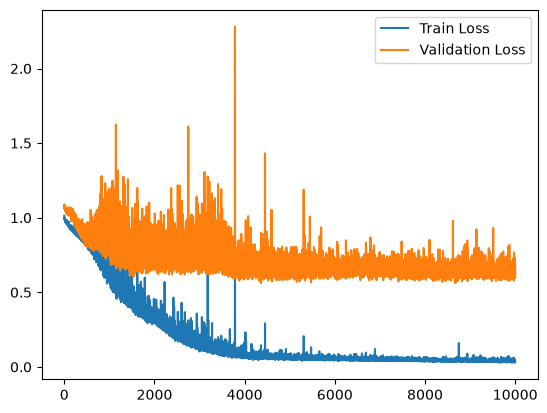
\includegraphics[width=\linewidth]{figures/loss_baseline.png}
    \caption{Curva de convergência da arquitetura baseline: decaimento acentuado no treino vs.\ estagnação turbulenta na validação.}
    \label{fig:loss_baseline}
\end{subfigure}
\hfill
\begin{subfigure}[t]{0.48\textwidth}
    \centering
    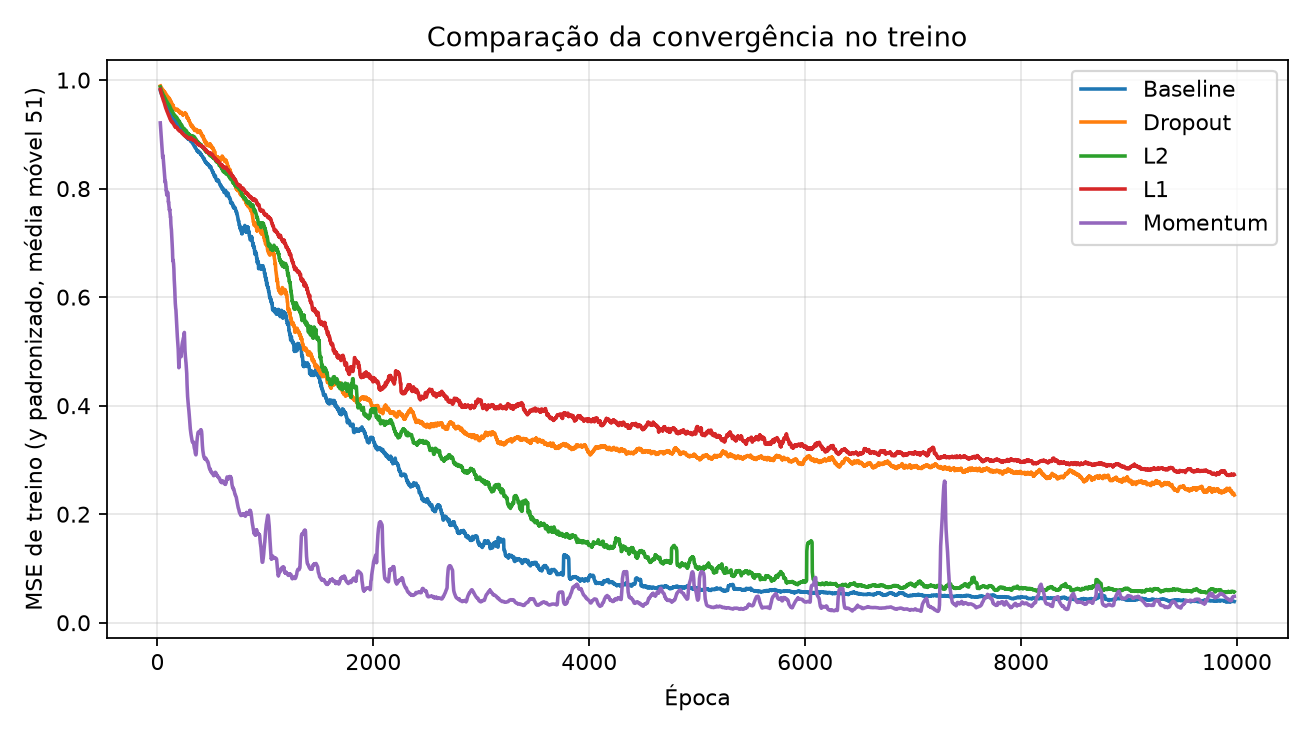
\includegraphics[width=\linewidth]{figures/loss_train_compare.png}
    \caption{MSE de treino suavizado por média móvel (janela 51): comparação de taxas de descida e patamares assintóticos.}
    \label{fig:loss_train}
\end{subfigure}
\caption{Dinâmica de aprendizado e convergência comparativa no subconjunto de treino.}
\label{fig:convergencia_geral}
\end{figure}

A análise comparativa do MSE de treino suavizado (Figura~\ref{fig:loss_train}) elucida os mecanismos operacionais de cada técnica. O modelo auxiliado pelo momento clássico de Polyak ($\beta = 0{,}9$) exibe uma aceleração convectiva drástica nas etapas iniciais, reduzindo o erro para valores inferiores a $0{,}20$ em menos de 500 épocas e atingindo o menor erro assintótico de treino ($\approx 0{,}039$). Contudo, a curva com momentum apresenta picos esporádicos de desestabilização (como próximo às épocas 2.000 e 7.200), causados pelo acúmulo de inércia vetorial que projeta os parâmetros para fora de desfiladeiros estreitos na superfície de perda. Em contrapartida, a regularização L2 ($\lambda = 10^{-3}$) acompanha a trajetória estável do baseline com decaimento controlado, convergindo suavemente para o patamar de $0{,}053$. Esse ligeiro incremento na perda de treino reflete a ação contínua da penalidade quadrática sobre os pesos, a qual restringe a norma euclidiana das conexões sem asfixiar a capacidade funcional da rede.

Em nítida oposição ao comportamento de L2 e do baseline, as curvas referentes a Dropout ($p = 0{,}05$) e L1 ($\lambda = 10^{-3}$) estabilizam-se em patamares substancialmente elevados de erro de treino ($0{,}222$ e $0{,}254$, respectivamente). No caso do Dropout, a anulação aleatória de 5\% das ativações neurais durante cada passagem direta (\textit{forward pass}) introduz um ruído multiplicativo estocástico que impede a rede de interpolar os 30 pontos de treinamento, forçando um subajuste artificial. Já na regularização L1, a derivada de magnitude constante aplicada aos pesos ($\lambda\,\mathrm{sgn}(W)$) força coeficientes menores a colapsarem bruscamente para zero, gerando esparsidade forçada que desativa canais essenciais de transmissão de informação em uma arquitetura densa.

\begin{figure}[htbp]
\centering
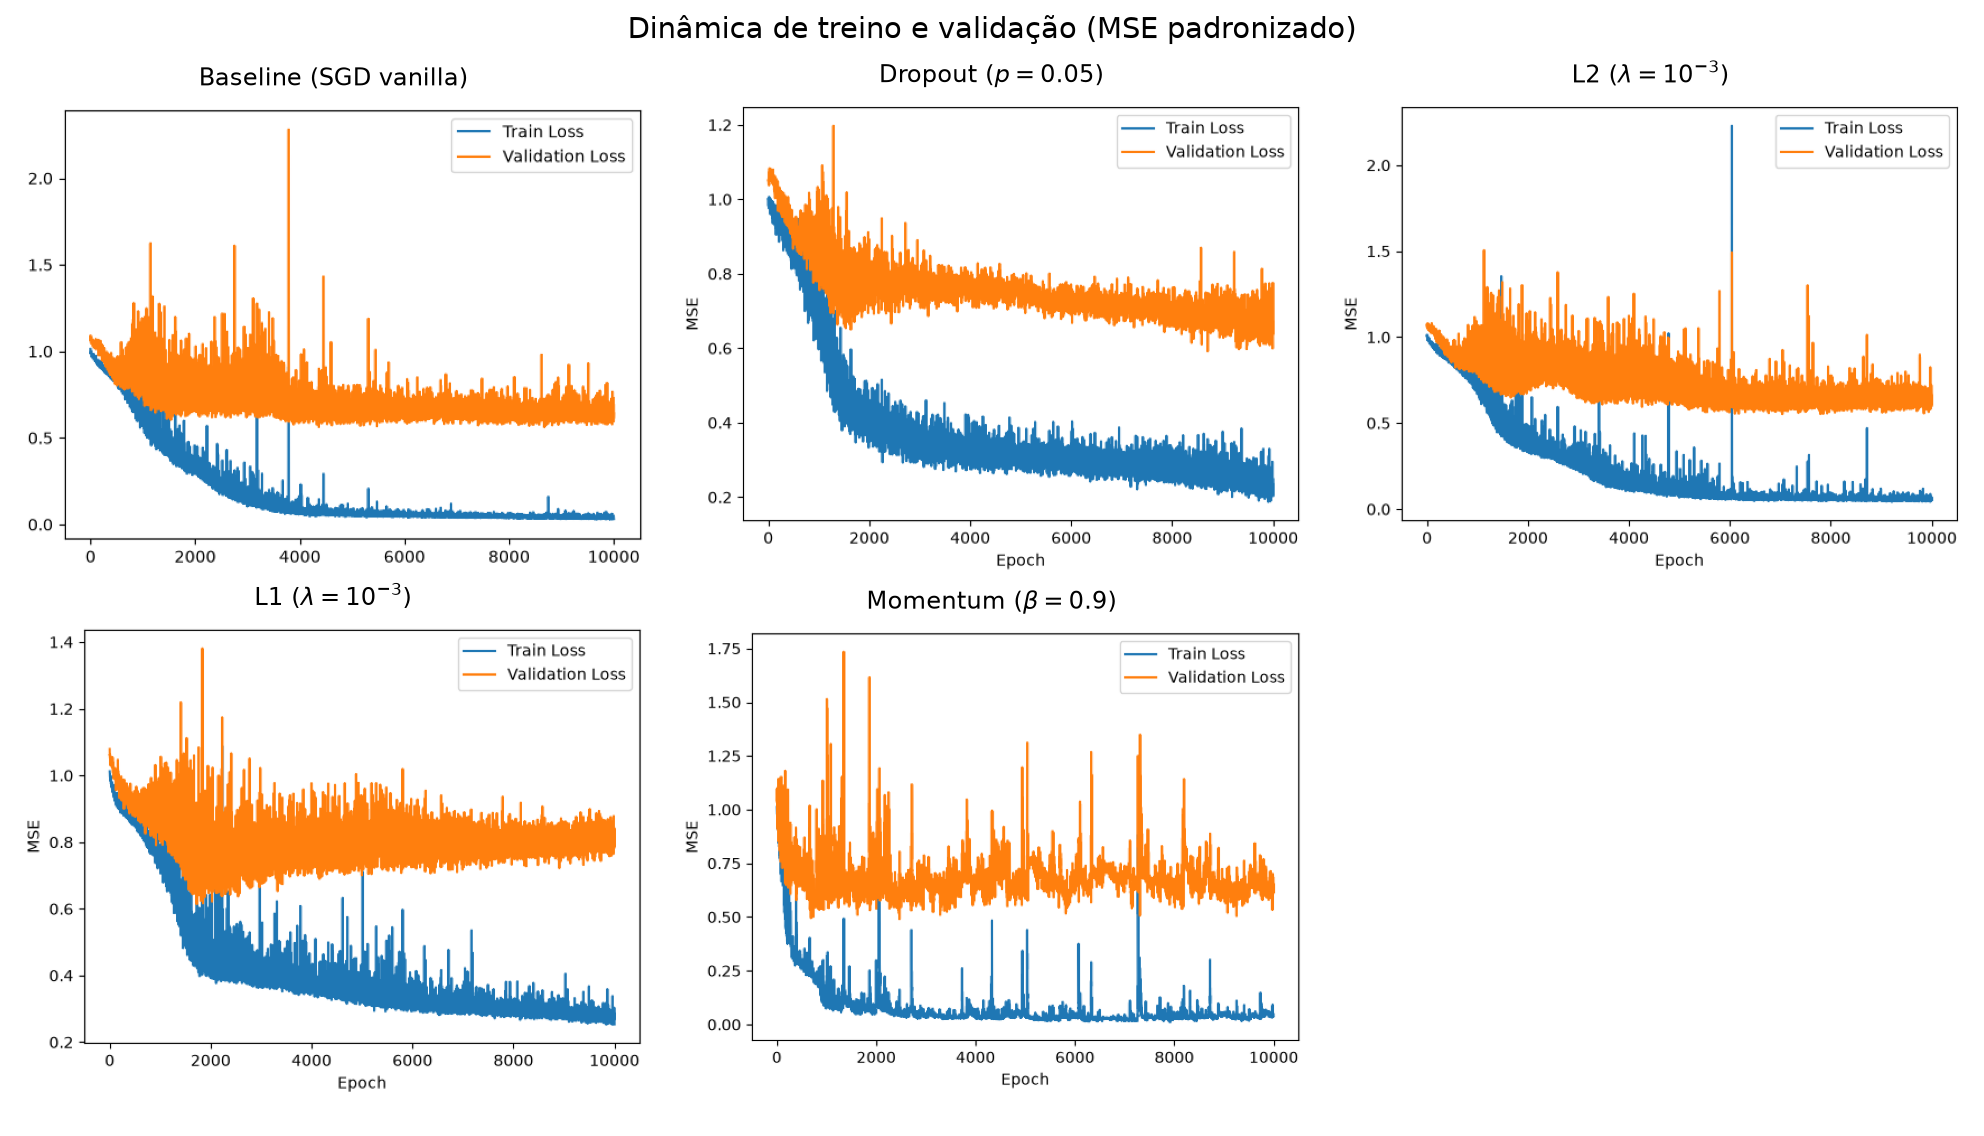
\includegraphics[width=0.80\textwidth]{figures/loss_ablation.png}
\caption{Painéis comparativos de treino e validação ao longo de 10.000 épocas para as cinco arquiteturas investigadas no estudo de ablação (MSE padronizado).}
\label{fig:loss_ablation}
\end{figure}

O painel global da dinâmica treino versus validação (Figura~\ref{fig:loss_ablation}) revela uma lição teórica essencial sobre a métrica de hiato de generalização: a aproximação das curvas de treino e validação não constitui, isoladamente, garantia de aprimoramento preditivo. Embora o Dropout exiba o menor hiato numérico absoluto da Tabela~\ref{tab:train_val} ($0{,}448$, comparado a $0{,}609$ do baseline), essa contração decorre exclusivamente da elevação do erro de treino, enquanto a perda de validação permanece em patamares insatisfatórios ($0{,}670$). Da mesma forma, a variante com L1 apresenta ruído persistente em ambas as curvas ao longo de todo o treinamento, estacionando na pior perda de validação entre todos os modelos ($0{,}791$). O otimizador com momentum atinge o ponto de mínimo de validação precocemente na época 2.470 (contra a época 8.673 do baseline), mas perpetua flutuações de alta amplitude até o encerramento do treino, mantendo o hiato de sobreajuste inalterado ($0{,}596$). A regularização L2, por sua vez, demonstrou ser a única estratégia capaz de promover simultaneamente a redução da perda de validação para $0{,}601$ e uma moderação controlada do sobreajuste.

\section{Estudo de Ablação e Avaliação no Conjunto de Teste}

O estudo de ablação foi estruturado segundo o princípio do isolamento estrito de variáveis, mantendo-se idênticas a topologia de camadas, a partição amostral, a taxa de aprendizado, o tamanho de lote e o número total de épocas. Foram avaliadas quatro modificações elementares frente ao baseline: a incorporação de inércia cinemática via Momentum ($\beta = 0{,}9$), o decaimento quadrático de pesos via Regularização L2 ($\lambda = 10^{-3}$), a penalização de esparsidade via Regularização L1 ($\lambda = 10^{-3}$, incidindo exclusivamente sobre matrizes de pesos), e a injeção de ruído estrutural estocástico via Dropout ($p = 0{,}05$ após cada camada ReLU). A avaliação empírica final foi realizada sobre as 240 amostras do conjunto de teste independente, convertendo-se as predições para a escala dimensional original de $y$. Os resultados quantitativos, incluindo o índice de época no qual a perda de validação atingiu seu ponto de mínimo retrospectivo (\textit{early stopping retrospectivo}), estão consolidados na Tabela~\ref{tab:ablation_metrics}.

\begin{table}[htbp]
\centering
\small
\renewcommand{\arraystretch}{1.25}
\caption{Resultados comparativos do estudo de ablação no conjunto de teste independente (240 amostras, escala dimensional original de $y$). A coluna temporal registra a época de convergência ótima na partição de validação.}
\label{tab:ablation_metrics}
\begin{tabularx}{\textwidth}{l c c c c >{\centering\arraybackslash}X}
\toprule
\textbf{Modelo / Variação Avaliada} & \textbf{MSE} & \textbf{RMSE} & \textbf{MAE} & \boldmath{$R^2$} & \textbf{Época do Mínimo ($\mathrm{val}$)} \\
\midrule
Baseline Vanilla (SGD puro) & 0{,}3383 & 0{,}5816 & 0{,}4633 & 0{,}3628 & 8673 \\
Baseline + Momentum ($\beta = 0{,}9$) & 0{,}3618 & 0{,}6015 & 0{,}4730 & 0{,}3186 & 2470 \\
\textbf{Baseline + L2 ($\lambda = 10^{-3}$)} & \textbf{0{,}3109} & \textbf{0{,}5576} & \textbf{0{,}4369} & \textbf{0{,}4143} & 7041 \\
Baseline + L1 ($\lambda = 10^{-3}$) & 0{,}4395 & 0{,}6629 & 0{,}5157 & 0{,}1722 & 1727 \\
Baseline + Dropout ($p = 0{,}05$) & 0{,}3886 & 0{,}6234 & 0{,}4918 & 0{,}2680 & 8704 \\
\bottomrule
\end{tabularx}
\end{table}

A regularização L2 consagrou-se como a única modificação capaz de superar o desempenho de generalização do baseline em todos os indicadores métricos: o coeficiente de determinação atingiu $R^2 = 0{,}4143$ (um ganho relativo de 14,2\% sobre os $0{,}3628$ do modelo base), enquanto o $\mathrm{MSE}$ foi reduzido de $0{,}3383$ para $0{,}3109$, o $\mathrm{RMSE}$ para $0{,}5576$ e o $\mathrm{MAE}$ para $0{,}4369$. A contração homogênea imposta pelo decaimento de pesos comprime as matrizes sinápticas em direção à origem do espaço vetorial, impedindo que derivadas locais atinjam grandezas desproporcionais para interpolar espuriamente ruídos do conjunto de treino. Ao suavizar o relevo funcional sem desconectar nós da rede, o operador L2 preserva a capacidade de aproximação global da MLP, atenuando a variância do estimador e alcançando o melhor equilíbrio no dilema viés-variância.

Em contraste com a regularização L2, a imposição da penalidade L1 provocou colapso severo no desempenho de teste, registrando $\mathrm{MSE} = 0{,}4395$ e $R^2 = 0{,}1722$ --- patamar estatisticamente equivalente ao alcançado por um polinômio linearmente ajustado sobre todo o domínio. Como a norma $\ell_1$ aplica uma taxa de atrito invariante sobre os pesos ($\Delta w_i \propto -\lambda\,\mathrm{sgn}(w_i)$), sinapses de magnitude moderada, cruciais para a transmissão não linear em arquiteturas univariadas estreitas, são sumariamente zeradas. Esse efeito restritivo asfixia a expressividade da rede e induz um falso mínimo de validação precoce na época 1.727, o qual reflete a transição precoce para um platô rígido de subajuste, e não um estado de otimização proveitoso.

O Dropout com taxa conservadora de descarte ($p = 0{,}05$) igualmente deteriorou a generalização no teste independente, obtendo $R^2 = 0{,}2680$ e $\mathrm{MSE} = 0{,}3886$. Embora o Dropout represente um paradigma consagrado para desarticular coadaptações em grandes conjuntos de dados, sua aplicação em regimes de reduzidíssima densidade amostral ($N_{\mathrm{treino}} = 30$) demonstra-se inadequada. A perturbação estocástica das ativações adiciona variância de amostragem interna excessiva em um cenário no qual as representações latentes já são frágeis. Em vez de operar como um ensemble regularizador, o mascaramento aleatório mutila a coerência dos padrões aprendidos, impedindo a rede de capturar satisfatoriamente o sinal determinístico subjacente.

Por fim, a incorporação de Momentum ($\beta = 0{,}9$) antecipou drasticamente a época de melhor validação para 2.470 iterações (redução temporal de 71,5\% frente às 8.673 épocas do baseline), mas resultou em ligeira degradação nos erros de generalização no teste ($\mathrm{MSE} = 0{,}3618$ e $R^2 = 0{,}3186$). Por constituir uma técnica puramente cinemática voltada ao condicionamento do trajeto de otimização, o momentum não estabelece qualquer restrição de capacidade ou penalização estrutural no espaço de hipóteses. Em cenários com amostras restritas e gradientes ruidosos, a inércia acelera indiscriminadamente tanto o aprendizado do sinal quanto a absorção de ruídos amostrais, propagando o modelo com rapidez para bacias de sobreajuste.

\section{Diagnóstico Residual, Análise Gráfica e Limitações Estruturais}

A inspeção diagnóstica dos modelos por meio de diagramas de dispersão de paridade (\textit{parity plots}) no conjunto de teste independente (Figura~\ref{fig:parity}) fornece uma confirmação visual da superioridade do modelo com decaimento de pesos L2 sobre o \textit{baseline}. Em ambas as configurações, os pontos dispersam-se ao longo da bissetriz ideal $y = \hat{y}$, comprovando que a rede neural conseguiu identificar a estrutura subjacente do processo gerador a despeito da correlação linear nula inicial. Todavia, a comparação direta evidencia que o modelo regularizado com L2 exibe um adensamento perceptivelmente mais compacto em torno da reta de identidade, sobretudo no intervalo central de maior densidade probabilística ($y \in [0, 1]$). O modelo baseline vanilla apresenta maior espalhamento lateral, sintoma direto da alta variância decorrente da memorização irrestrita. Em ambos os casos, observa-se maior dispersão nas extremidades do domínio ($y < -0{,}5$ e $y > 1{,}5$), padrão atribuível à baixa densidade de observações nas caudas da distribuição original e aos efeitos de borda característicos da aproximação por funções de base localizadas.

\begin{figure}[htbp]
\centering
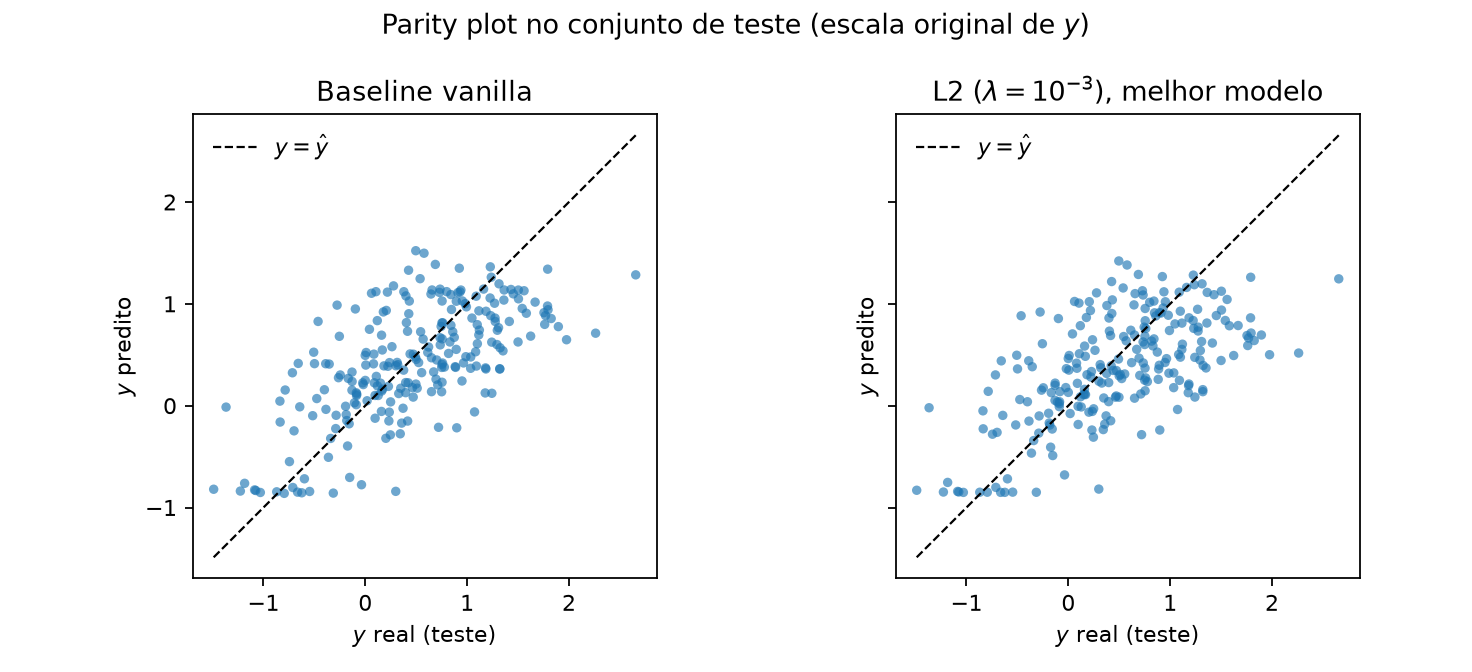
\includegraphics[width=0.66\textwidth]{figures/parity.png}
\caption{Diagrama de paridade no conjunto de teste (escala dimensional original de $y$): dispersão entre valores reais e predições para a MLP Baseline Vanilla (esquerda) e para a MLP com regularização L2 (direita).}
\label{fig:parity}
\end{figure}

O diagnóstico detalhado dos resíduos de predição do modelo L2 ($e = y - \hat{y}$), apresentado na Figura~\ref{fig:residuals}, corrobora a consistência estatística do regressor ótimo. No gráfico de resíduos em função dos valores preditos $\hat{y}$ (esquerda), a nuvem de pontos distribui-se de maneira aleatória e uniforme em torno da linha de erro nulo ($e = 0$), sem exibir qualquer conformação curvilínea remanescente (como perfis parabólicos ou senoidais). Essa dispersão desprovida de padrão estrutural atesta que a rede de três camadas capturou integralmente a componente determinística não linear da função geradora, não restando vieses sistemáticos não modelados. Ademais, a largura vertical da faixa residual permanece estável ao longo de toda a amplitude predita ($\hat{y} \in [-0{,}8,\, 1{,}5]$), caracterizando uma aproximação satisfatória da hipótese de homocedasticidade (variância residual constante).

\begin{figure}[htbp]
\centering
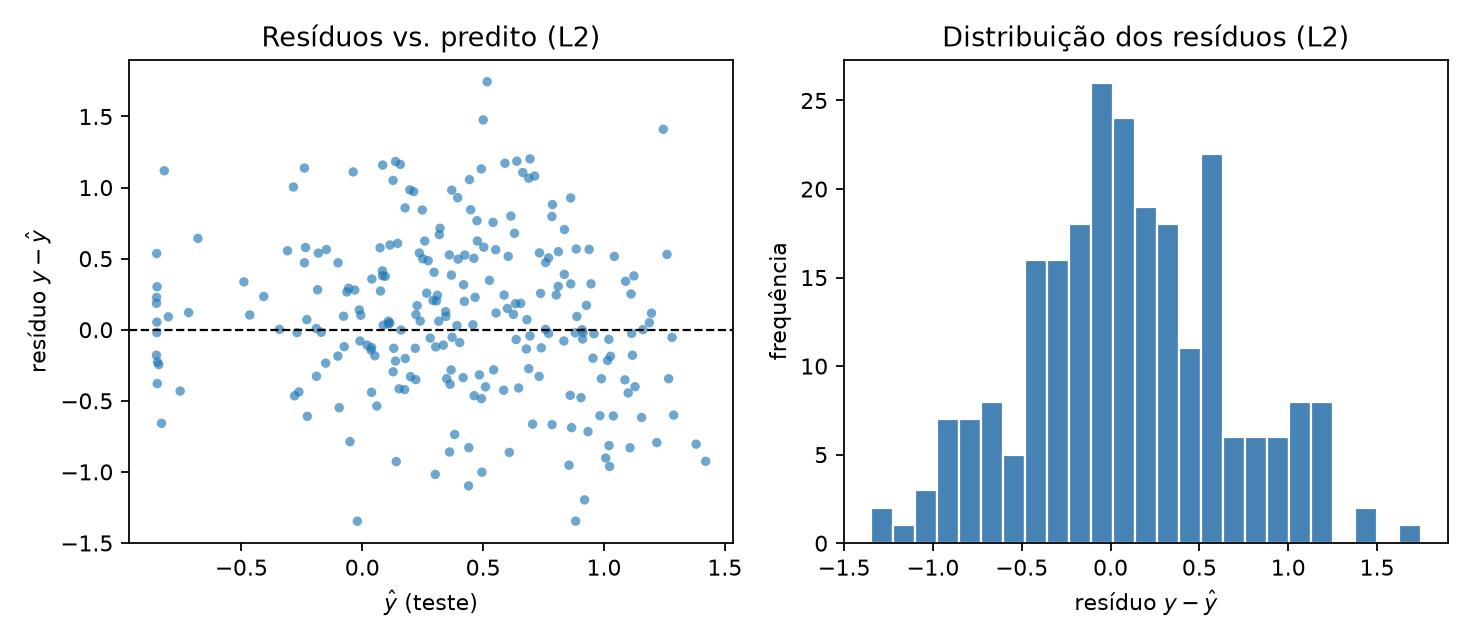
\includegraphics[width=0.66\textwidth]{figures/residuals.png}
\caption{Diagnóstico estatístico dos resíduos da MLP com regularização L2 no conjunto de teste independente: gráfico de dispersão de resíduos vs.\ predição (esquerda) e histograma de distribuição residual (direita).}
\label{fig:residuals}
\end{figure}

A distribuição empírica dos resíduos ilustrada no histograma da Figura~\ref{fig:residuals} (direita) exibe formato unimodal, aproximadamente simétrico e campanulado, assemelhando-se a uma distribuição gaussiana centrada em zero ($\mu_{\mathrm{res}} \approx 0$). A moda da distribuição situa-se precisamente no intervalo nulo, com densidade predominante contida na faixa de $[-0{,}5,\, 0{,}5]$ e caudas simétricas que se estendem até $[-1{,}5,\, 1{,}5]$. Uma dedução quantitativa direta permite avaliar o quão próximo o modelo se encontra do limite teórico estocástico do problema. Sabendo-se que o desvio-padrão amostral da variável alvo original é $\sigma_y \approx 0{,}7267$ (variância total $\sigma_y^2 \approx 0{,}5281$) e que o modelo L2 alcançou coeficiente de determinação $R^2 = 0{,}4143$, a proporção de variância não explicada equivale a $1 - R^2 = 0{,}5857$. A estimativa teórica do desvio-padrão do ruído residual remanescente é dada por $\sigma_{\mathrm{res}} = \sigma_y \sqrt{1 - R^2} = 0{,}7267 \times \sqrt{0{,}5857} \approx 0{,}5561$, grandeza que coincide de forma notável com o erro quadrático médio da raiz observado empiricamente no teste ($\mathrm{RMSE} = 0{,}5576$). Esse alinhamento demonstra que o erro do modelo L2 é governado majoritariamente pela variância do ruído estocástico intrínseco do processo gerador, e não por insuficiência representacional da arquitetura neural.

Entre as limitações metodológicas identificadas no desenho experimental, ressalta-se o protocolo de parada antecipada (\textit{early stopping}): embora a coluna de épocas da Tabela~\ref{tab:ablation_metrics} reporte retrospectivamente o argmin do erro de validação, os pesos efetivamente avaliados no conjunto de teste correspondem aos estados consolidados ao término da época 10.000. No caso do modelo L2, que alcançou seu mínimo ótimo de validação na época 7.041, a restauração direta dos pesos daquele ponto específico poderia propiciar ganhos marginais adicionais de generalização. Outro aspecto relevante concerne à avaliação orientada por uma única partição aleatória: embora garanta estrita reprodutibilidade, a estimativa pontual pode carregar variabilidade amostral específica da semente 123, sendo recomendável em trabalhos futuros o cômputo de médias e desvios por validação cruzada estratificada em $k$-dobras (\textit{$k$-fold cross-validation}).

\section{Conclusões e Considerações Finais}

A investigação experimental conduzida neste trabalho elucidou com clareza o comportamento de redes neurais do tipo Perceptron Multicamadas quando submetidas a cenários extremos de escassez de dados ($N \ll p$), no qual a capacidade paramétrica da arquitetura supera em ordens de magnitude o número de instâncias de ajuste. O modelo baseline puramente estocástico confirmou a propensão inata de modelos superparametrizados a memorizar ruídos empíricos, atingindo perdas de treino próximas a zero e estagnando em perdas elevadas de validação e teste.

O estudo sistemático de ablação demonstrou que diferentes classes de intervenções algorítmicas exercem impactos estruturalmente discrepantes sobre a generalização. A regularização por decaimento de pesos L2 ($\lambda = 10^{-3}$) destacou-se categoricamente como a melhor formulação, atenuando as magnitudes dos pesos e restringindo a curvatura local da função de regressão de forma contínua, o que elevou o coeficiente $R^2$ no teste para $0{,}4143$. Em contraste, estratégias baseadas em descarte estocástico de neurônios (Dropout) e indução de esparsidade absoluta (L1) mostraram-se inadequadas para o regime de pequeno volume amostral, introduzindo perturbações excessivas e amputando representações latentes indispensáveis, o que culminou em severo subajuste. Ademais, evidenciou-se que otimizadores com termo de momento aceleram intensamente a convergência ao custo potencial de antecipar a memorização de ruído, não substituindo o papel de penalizadores explícitos de complexidade. A concordância estrita entre o RMSE de teste e o desvio-padrão teórico do ruído do conjunto de dados ratifica que a solução obtida com a regularização L2 alcançou o patamar de desempenho ótimo viável para o problema proposto.

\end{document}
